% ------------------------------------------------------------------------------
\clearpage
\section{Multivariate Analysis}
% ------------------------------------------------------------------------------

\begin{figure}[htbp]
  \centering

  \begin{subfigure}[t]{.49\textwidth}
    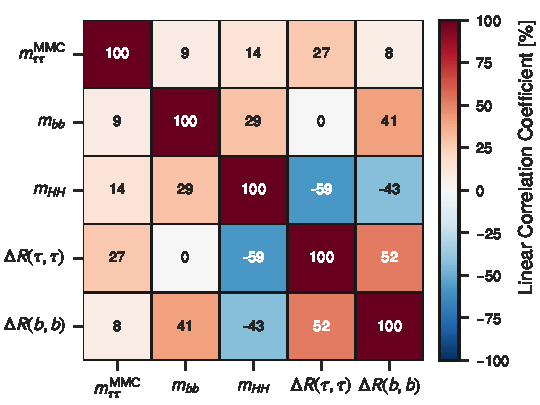
\includegraphics[width=\textwidth]{mva/correlations/NonResHH_pearson}
    \subcaption{SM \HH (gluon fusion)}
  \end{subfigure}\hfill %
  \begin{subfigure}[t]{.49\textwidth}
    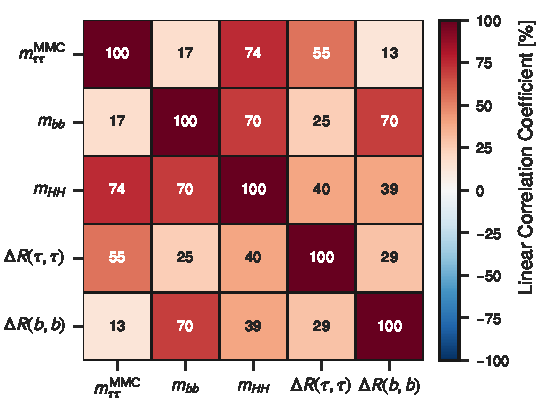
\includegraphics[width=\textwidth]{mva/correlations/ttbar_pearson}
    \subcaption{\ttbar}
  \end{subfigure}

  \begin{subfigure}[t]{.49\textwidth}
    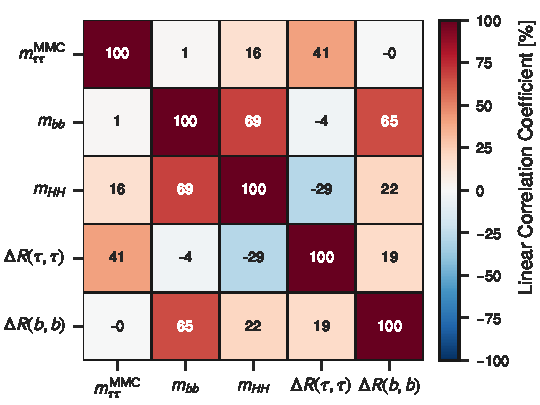
\includegraphics[width=\textwidth]{mva/correlations/Ztautau_pearson}
    \subcaption{$Z \rightarrow \tautau + \text{jets}$}
  \end{subfigure}\hfill %
  \begin{subfigure}[t]{.49\textwidth}
    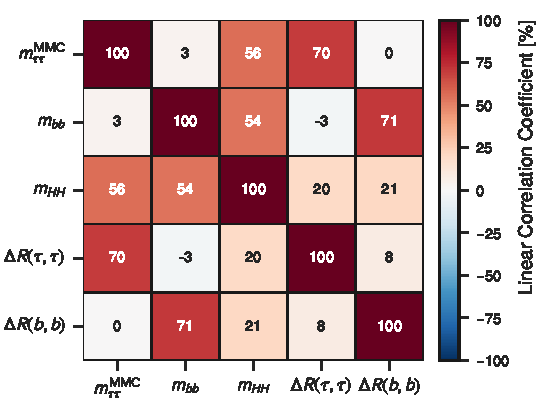
\includegraphics[width=\textwidth]{mva/correlations/Fake_pearson}
    \subcaption{Multi-jet}
  \end{subfigure}

  \caption{Correlation matrices of the MVA input variables for the SM
    \HH signal and the three largest background contributions (b) -
    (d) in the \hadhad SR.}
  \label{fig:mva_input_correlations}
  \todo[inline]{Will move to appendix (or remove completely).}
\end{figure}



% ------------------------------------------------------------------------------
\clearpage
\subsection{Description of Discriminating Variables used in the
  \lephad Channels}%
\label{app:lephad_mva_variables}
% ------------------------------------------------------------------------------

A description of variables used in the \lephad channels is given in
the following.  Reconstructed electrons and muons are collectively
referred to as leptons ($\ell$).
\begin{description}

\item[$\Delta \pT(\ell, \tauhadvis)$] The transverse momentum
  difference between lepton and \tauhadvis.

\item[\mTW] Transverse mass of the \PW boson for processes where
  \pTmiss solely originates from the decay $\PW \ra \ell \nu_\ell$ defined as:
  $\mTW = \sqrt{2 |\pT^{\ell}| |\pTmiss| \cos(1 - \Delta\phi)}$.

\item[\pTmiss $\phi$ centrality] A measure of the relative angular
  position of \pTmiss and visible \taulepton decay products
  (electrons, muons, or \tauhadvis) in the transverse plane. It is
  defined as~\cite{HIGG-2013-32, HIGG-2016-16-witherratum}:
  % The
  % measurement is relative to the line bisecting the azimuthal angle
  % between the pair of visible \taulepton decay products and is defined
  % as~\cite{HIGG-2013-32, HIGG-2016-16-witherratum}:
  \begin{align*}
    \pTmiss\text{ }\phi\text{ centrality} = \frac{A + B}{\sqrt{A^2 + B^2}} \text{,}
  \end{align*}
  where
  \begin{align*}
    A = \frac{\sin(\phi_{\pTmiss} - \phi_{\tau_1})}{\sin(\phi_{\tau_2} - \phi_{\tau_1})} \qquad B = \frac{\sin(\phi_{\tau_2} - \phi_{\pTmiss})}{\sin(\phi_{\tau_2} - \phi_{\tau_1})} \text{,}
  \end{align*}
  with $\phi_{\pTmiss}$ and $\phi_{\tau_1}$ / $\phi_{\tau_2}$ denoting
  the azimuthal angle of \pTmiss and visible \taulepton decay
  products, respectively.

  The \pTmiss $\phi$ centrality is defined relative to the line
  bisecting the azimuthal angle spanned by the visible \taulepton
  decay products. It reaches a maximum of $\sqrt{2}$ (minimum of
  $-\sqrt{2}$) when \pTmiss is aligned with the bisecting line and
  pointing into the smaller (larger) angle defined by the decay
  products. In configurations where \pTmiss is collinear with one of
  the visible \taulepton decay products it takes a value of 1.

\item[$\Delta\phi(\ell\tauhadvis, bb)$] Azimuthal angle between the
  $\ell + \tauhadvis$ system and the system consisting of the two
  \bjet candidates.

\item[$\Delta\phi(\ell, \pTmiss)$] Azimuthal angle between the lepton
  and \pTmiss.

\item[$\Delta\phi(\pTauTau, \pTmiss)$] Azimuthal angle between
  $\tau\tau$-system, reconstructed using the MMC, and \pTmiss.

\item[$s_{\text{T}}$] The effective mass of the event defined as the
  scalar sum of transverse momenta of all selected jets, \tauhadvis,
  leptons, and \pTmissAbs.
\end{description}

% ------------------------------------------------------------------------------
\clearpage
\subsection{Discrimination Power of the PNN as a Function of \mX}%
\label{app:pnn_rocauc_vs_mx}
% ------------------------------------------------------------------------------

\begin{figure}[htbp]
  \centering

  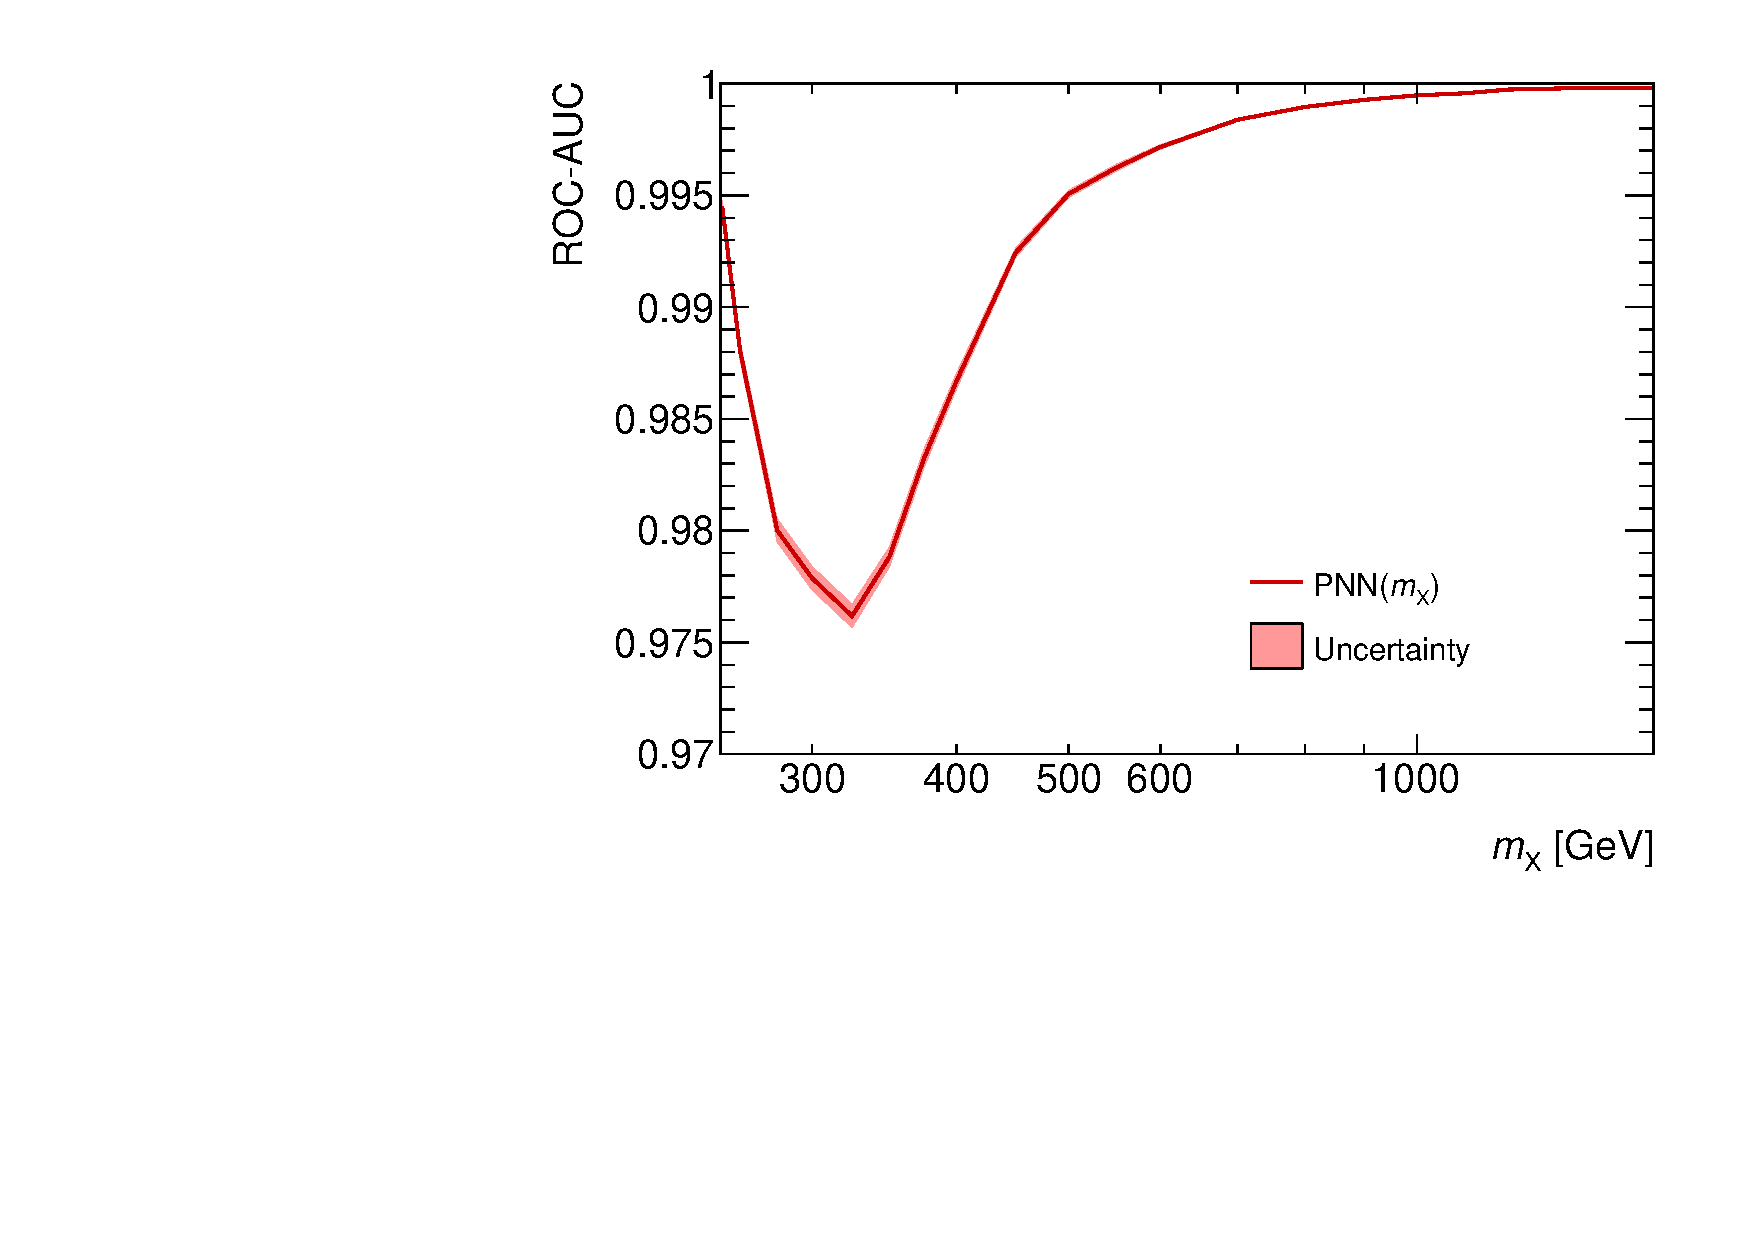
\includegraphics[width=0.6\textwidth]{mva/rocauc_vs_mx}

  \caption{Area under the receiver operating curve (ROC-AUC) for the
    PNN classifier used for the search for resonant \HH production in
    the \hadhad channel. The ROC-AUC is shown for the PNN after
    hyperparameter optimisation as a function of the signal hypothesis
    (specified by \mX). Only statistical uncertainties are shown.}%
  \label{fig:pnn_rocauc_vs_mx}
\end{figure}


%%% Local Variables:
%%% mode: latex
%%% TeX-master: "../../phd_thesis"
%%% End:
